\documentclass[11pt]{article}

\usepackage[a4paper,margin=1in]{geometry}
\usepackage{amsmath,amssymb,amsthm,mathtools}
\usepackage{bm}
\usepackage{booktabs}
\usepackage{graphicx}
\usepackage{hyperref}
\usepackage[numbers]{natbib}
\usepackage{tikz-cd}

\newcommand{\ones}{\mathbf{1}}
\newcommand{\diag}{\operatorname{diag}}
\newcommand{\KL}{\operatorname{KL}}
\newcommand{\Kset}{\mathcal{K}}
\newcommand{\Piset}{\Pi}
\newtheorem{proposition}{Proposition}

\title{Tutorial on Discrete Diffusion}
\author{Gabriel Peyr\'e\\gabriel.peyre@ens.fr\\CNRS and PSL Universit\'e}
\date{April 9, 2026}

\begin{document}
\maketitle

\begin{abstract}
These notes are a companion mathematical tutorial to the Jupyter notebook ``Discrete Diffusion'', available at \url{https://github.com/gpeyre/ot4ml}. They focus mostly on diffusion models in discrete space and discrete time. The guiding question is how to learn a generative procedure that maps samples from a simple reference distribution toward an unknown target distribution when one only has access to finitely many samples from the target law. Throughout most of the notes, the interpolant is assumed to be a Markov process, which leads in discrete space to the learning of reverse transition kernels. This Markovian assumption is natural for diffusion models, but the same general viewpoint can be extended to arbitrary interpolants, in which case one obtains the analogue of flow matching in place of denoising score matching.
\end{abstract}

\section{Question Addressed by Diffusion Models in Discrete Space}
One starts from an unknown target distribution $h^0$ on a finite state space. In practice, one does not know the density $h^0$ explicitly: one only has access to $N_0$ samples drawn from it. The objective is to generate new samples distributed approximately according to $h^0$ without first performing a full density-estimation step. Diffusion models provide an algorithmic route to do so by learning a parametric map from a simple reference distribution $h^\infty$ back to the data distribution $h^0$.

In continuous space, this reverse map is often represented by an advection vector field and can therefore be implemented through a deterministic flow once noise is added at the infinitesimal level. In discrete space the situation is more brute-force: because mass must in general be split between several states, one cannot rely on a purely deterministic map. One instead learns a reverse transition kernel sending samples from a simple terminal law toward samples from $h^0$.

\section{Forward Noising Process}
The presentation in this section is inspired in particular by \citet{austin2021structured}, \citet{campbell2022continuous}, and \citet{pauline2025foundations}.

We work on a finite state space $\mathcal{X}=\{1,\dots,n\}$. Let
\[
h^t\in\mathbb{R}_+^n,\qquad \sum_{i=1}^n h_i^t=1
\]
be the histogram (marginal law) at time $t$.

The forward kernel is row-stochastic:
\[
P\in\mathbb{R}_+^{n\times n},\qquad P_{i,j}=\mathbb{P}(X_{t+1}=j\mid X_t=i),\qquad P\ones=\ones.
\]
Forward marginals follow
\begin{equation}
\label{eq:forward-recursion}
h^{t+1}=P^\top h^t,
\end{equation}
for $t=0,\dots,T-1$, hence we have $T+1$ histograms $(h^0,\dots,h^T)$.

\paragraph{Examples of forward kernels (detailed).}
\begin{itemize}
\item \textbf{Local geometric kernel.}
For interior states, mass is split on neighbors and self:
\[
P_{i,j}=\frac13\,\mathbf{1}_{j\in\{i-1,i,i+1\}},
\]
with boundary rows set by a chosen convention (reflecting or periodic).
This kernel encodes local motion and typically smooths histograms spatially.

\item \textbf{Gaussian convolution kernel.}
For a bandwidth $\sigma>0$,
\[
P_{i,j}\propto \exp\!\left(-\frac{(i-j)^2}{2\sigma^2}\right),
\qquad
\sum_j P_{i,j}=1.
\]
Large $\sigma$ gives stronger global mixing; small $\sigma$ remains local.

\item \textbf{Masking/absorbing kernel.}
Choose a special absorbing state $n$ and set
\[
P_{i,i}=1-\varepsilon,\quad P_{i,n}=\varepsilon\ (i\neq n),\quad P_{n,n}=1.
\]
The process progressively transfers mass toward state $n$.
\end{itemize}

\paragraph{Forward particle process.}
Define one Markov process $(X^t)_{t=0}^T$ by
\[
X^0\sim h^0,
\qquad
X^{t+1}\sim P\big(X^t,\cdot\big).
\]
Then
\[
h^t=\mathrm{Law}(X^t),
\]
and \eqref{eq:forward-recursion} is exactly the evolution of this law.

\paragraph{Forward figures.}
The script \texttt{figures/figures.py} generates forward visualizations using the same Gaussian forward kernel as the notebook,
\[
P_{i,j}\propto \exp\!\left(-\frac{(i-j)^2}{2\sigma^2}\right),\qquad \sigma=0.75.
\]
\begin{figure}[h]
\centering
\begin{minipage}{0.48\linewidth}
\centering
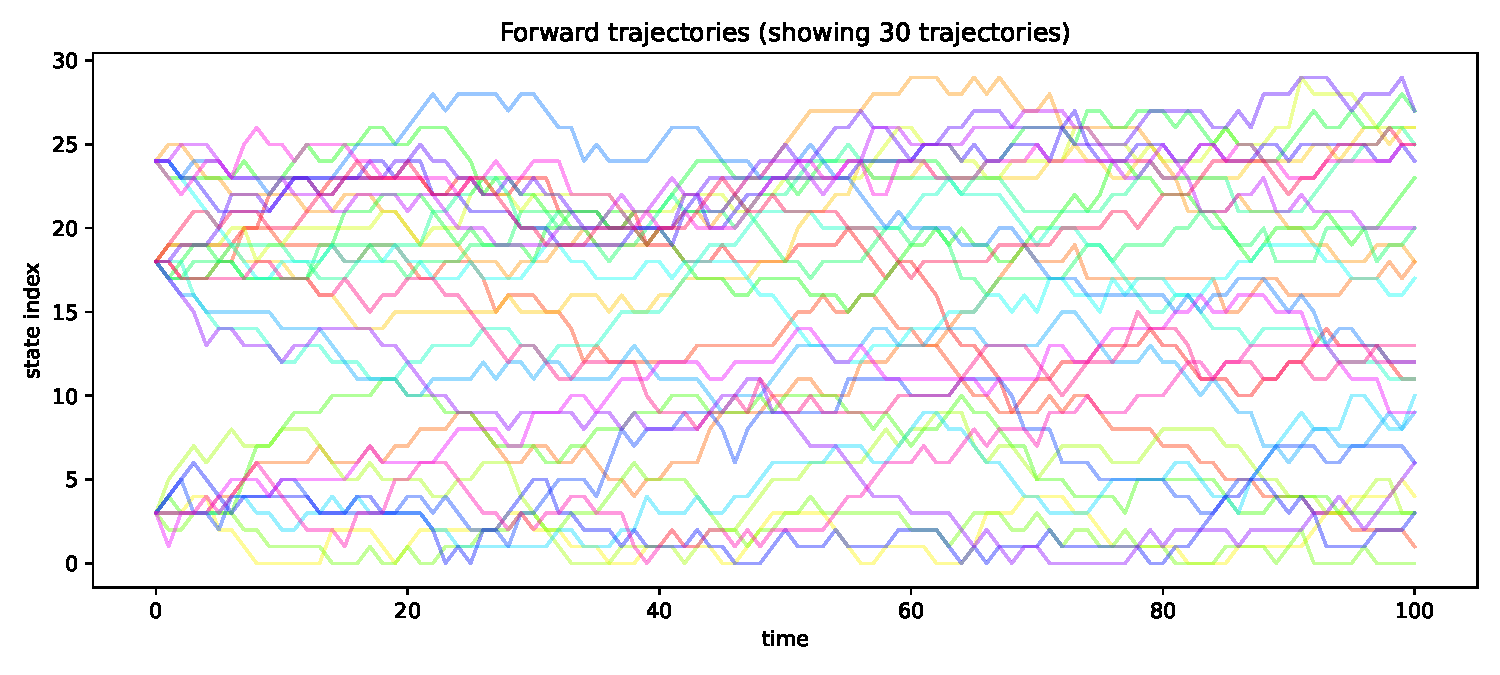
\includegraphics[width=\linewidth]{figures/forward_trajectories.pdf}
\end{minipage}\hfill
\begin{minipage}{0.48\linewidth}
\centering
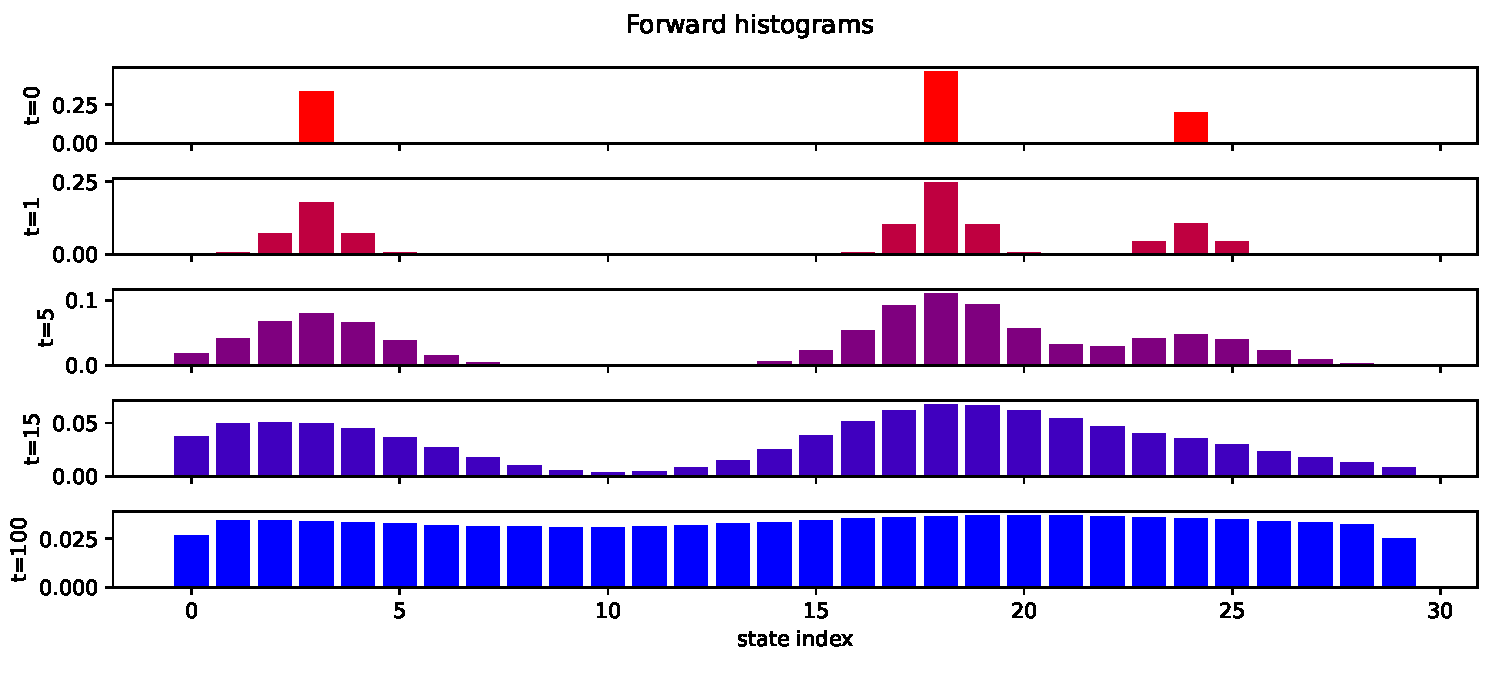
\includegraphics[width=\linewidth]{figures/forward_histograms.pdf}
\end{minipage}
\caption{Forward process (left: trajectories, right: vertically stacked histogram snapshots) generated with the Gaussian kernel $P$.}
\label{fig:forward-figures}
\end{figure}

\section{Backward Kernels and Coupling}
\subsection{Admissible kernels between consecutive marginals}
Fix $a,b\in\Delta_n$ (probability simplex). Define
\[
\Kset(a,b)=\left\{K\in\mathbb{R}_+^{n\times n}:\ K\ones=\ones,\ K^\top a=b\right\}.
\]
Thus $P\in\Kset(h^t,h^{t+1})$ by \eqref{eq:forward-recursion}.

An inverse (backward) kernel at step $t$ is any
\[
Q^t\in\Kset(h^{t+1},h^t),
\]
that is,
\[
Q^t\ones=\ones,
\qquad
(Q^t)^\top h^{t+1}=h^t.
\]
So there are exactly $T$ backward kernels $Q^0,\dots,Q^{T-1}$ connecting $t+1\to t$.

\subsection{Backward particle process}
Given admissible kernels $(Q^t)_{t=0}^{T-1}$, define $(Y^t)_{t=0}^T$ backward by
\[
Y^T\sim h^T,\qquad
Y^t\sim Q^t(Y^{t+1},\cdot),\quad t=T-1,\dots,0.
\]
If each $Q^t\in\Kset(h^{t+1},h^t)$, then
\[
\mathrm{Law}(Y^t)=h^t,\qquad t=0,\dots,T,
\]
so backward recursion terminates at $h^0$.

\subsection{Bayes inverse as a canonical admissible reverse kernel}
\paragraph{Definition (Bayes kernel).}
Given a forward chain with kernel $P$ and marginals $(h^t)$, the Bayes kernel at time $t$ is
\[
Q^{\mathrm B,t}_{j,i}\coloneqq
\mathbb{P}(X^t=i\mid X^{t+1}=j).
\]
This is to be contrasted with the forward convention
\[
P_{i,j}=\mathbb P(X^{t+1}=j\mid X^t=i).
\]

\begin{proposition}
Let $a=h^t$, $b=h^{t+1}$ and $P\in\Kset(a,b)$. Define the diagonal pseudo-inverse by
\[
b^+\coloneqq (b_i^+)_{i=1}^n,
\qquad
b_i^+=
\begin{cases}
1/b_i & \text{if } b_i>0,\\
0 & \text{if } b_i=0.
\end{cases}
\]
Then the Bayes kernel is given componentwise by
\begin{equation}
\label{eq:bayes-entry}
Q^{\mathrm B}_{j,i}=a_i P_{i,j}\, b_j^+.
\end{equation}
In matrix form,
\begin{equation}
\label{eq:bayes-diag}
Q^{\mathrm B}=\diag(b)^+P^\top\diag(a).
\end{equation}
Moreover, $Q^{\mathrm B}\in\Kset(b,a)$, i.e. it is an admissible inverse kernel.
\end{proposition}
\begin{proof}
The component formula is exactly Bayes rule when $b_j>0$, and the pseudo-inverse convention sets the corresponding row to zero when $b_j=0$. Since $b=P^\top a$, the latter case implies
\[
b_j=\sum_i a_i P_{i,j}=0,
\]
hence $a_i P_{i,j}=0$ for every $i$, so the formula is still consistent.

For admissibility, first compute
\[
Q^{\mathrm B}\ones
=
\diag(b)^+P^\top a
=
\diag(b)^+ b.
\]
For every $j$ such that $b_j>0$, the $j$-th entry equals $1$. If $b_j=0$, then the $j$-th row of $Q^{\mathrm B}$ is identically zero and this row is never visited under the marginal $b$; equivalently, the conditional law on that null-mass event is immaterial. On the support of $b$, $Q^{\mathrm B}$ is therefore stochastic.

Next,
\[
(Q^{\mathrm B})^\top b
=
\diag(a)P\diag(b)^+ b
=
\diag(a)P\mathbf 1
=
\diag(a)\mathbf 1
=
a.
\]
Hence $Q^{\mathrm B}$ is an admissible inverse kernel from $b$ to $a$.
\end{proof}

\paragraph{Bayesian inversion map.}
Define
\[
\mathcal B_{a,b}:\Kset(a,b)\to\Kset(b,a),\qquad
\mathcal B_{a,b}(K)\coloneqq \diag(b)^+K^\top\diag(a).
\]
On supports where $a_i,b_i>0$, this map is a bijection, with inverse
\[
\mathcal B_{a,b}^{-1}(L)=\mathcal B_{b,a}(L)=\diag(a)^+L^\top\diag(b).
\]
Therefore Bayesian inversion is not only a way to build one reverse kernel from $P$; it defines a one-to-one correspondence between admissible forward kernels and admissible backward kernels.

\paragraph{Backward figures.}
Using $Q^t=\mathcal B_{h^t,h^{t+1}}(P)$ at each step, the backward process
\[
Y^T\sim h^T,\qquad Y^t\sim Q^t(Y^{t+1},\cdot)
\]
has marginals $h^t$ for $t=T,\dots,0$. Figure~\ref{fig:backward-figures} displays backward trajectories (left) and empirical histograms of $Y^t$ (right), generated with the Bayes inverse kernels associated with the same Gaussian forward kernel $P$.
\begin{figure}[h]
\centering
\begin{minipage}{0.48\linewidth}
\centering
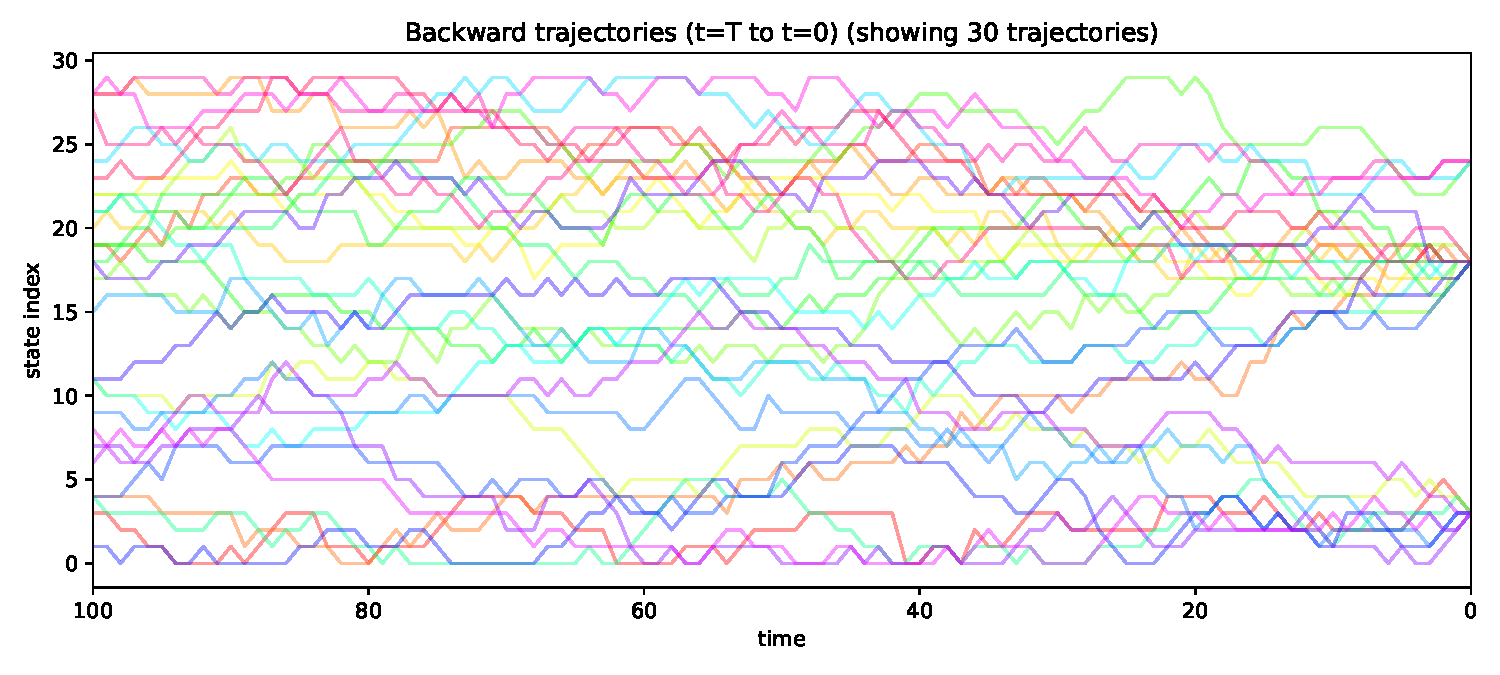
\includegraphics[width=\linewidth]{figures/backward_trajectories.pdf}
\end{minipage}\hfill
\begin{minipage}{0.48\linewidth}
\centering
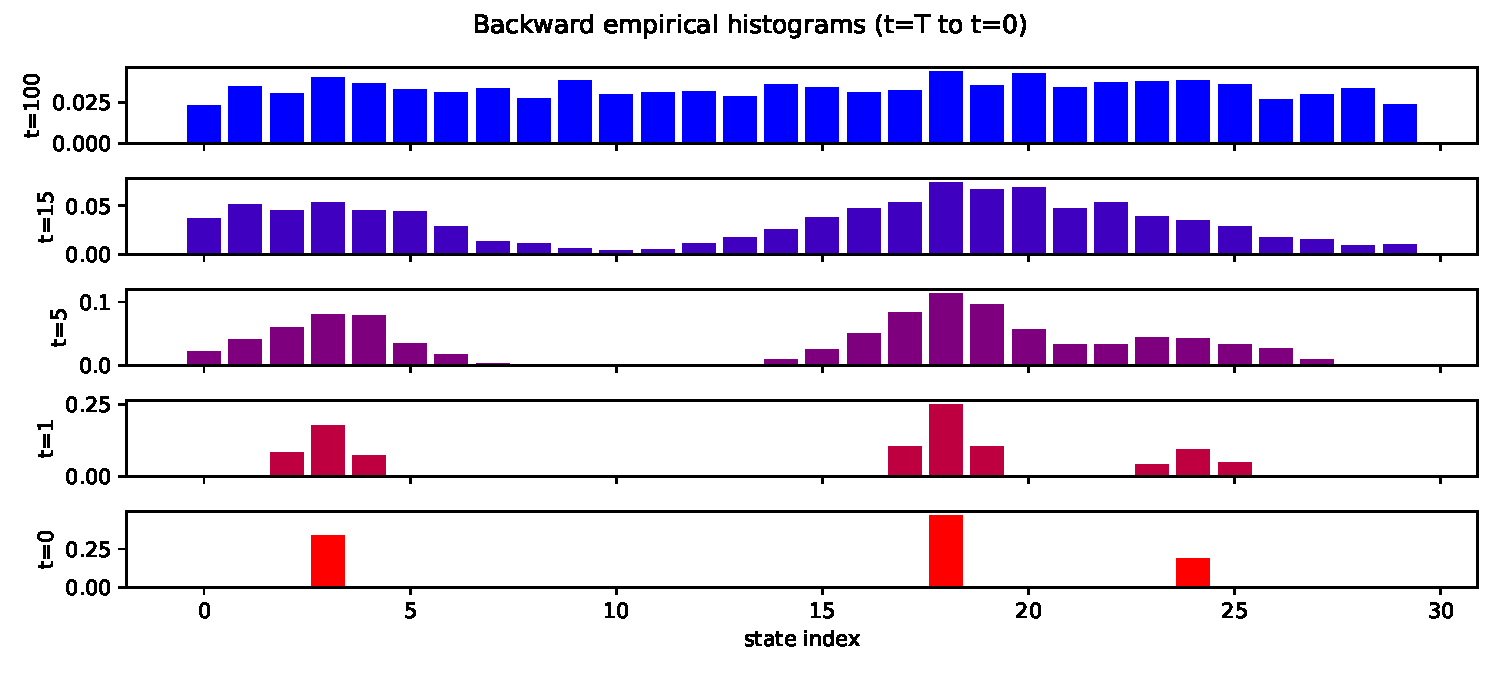
\includegraphics[width=\linewidth]{figures/backward_histograms.pdf}
\end{minipage}
\caption{Backward process (left: trajectories in backward time, right: vertically stacked empirical histogram snapshots of $Y_t$). Kernel: Bayes inverse of the Gaussian forward kernel $P$.}
\label{fig:backward-figures}
\end{figure}

\subsection{Coupling polytope and bijection with kernels}
Define
\[
\Piset(a,b)=\left\{\pi\in\mathbb{R}_+^{n\times n}:\ \pi\ones=a,\ \pi^\top\ones=b\right\}.
\]

\begin{proposition}[Kernel--coupling bijection]
Define
\[
\Phi_a:\Kset(a,b)\to\Piset(a,b),\qquad \Phi_a(K)=\diag(a)K.
\]
Then $\Phi_a$ is well-defined. Its inverse is
\[
\Phi_a^{-1}(\pi)=\diag(a)^+\pi,
\]
where $\diag(a)^+$ is the diagonal pseudo-inverse ($1/a_i$ if $a_i>0$, else $0$). In particular, choosing an admissible kernel in $\Kset(a,b)$ is equivalent to choosing a coupling in $\Piset(a,b)$.
\end{proposition}
\begin{proof}
Let $K\in\Kset(a,b)$ and set $\pi=\diag(a)K$. Since $\pi\geq 0$,
\[
\pi\ones=\diag(a)K\ones=\diag(a)\ones=a
\]
and
\[
\pi^\top \ones = K^\top a=b.
\]
Thus $\pi\in\Piset(a,b)$.

Conversely, let $\pi\in\Piset(a,b)$ and define $K=\diag(a)^+\pi$. Then $K\geq0$ and
\[
K^\top a=\pi^\top \diag(a)^+ a = \pi^\top \ones = b,
\]
while on the support of $a$,
\[
K\ones=\diag(a)^+\pi\ones=\diag(a)^+ a=\ones.
\]
Hence $K\in\Kset(a,b)$ up to the same null-mass convention as above, and the two formulas are inverse to each other.
\end{proof}

\begin{proposition}[Interleaving with transposition]
Let
\[
\mathsf T:\Piset(a,b)\to\Piset(b,a),\qquad \mathsf T(\pi)=\pi^\top.
\]
Define similarly
\[
\Phi_b:\Kset(b,a)\to\Piset(b,a),\qquad \Phi_b(L)=\diag(b)L.
\]
Then
\[
\mathsf T\circ \Phi_a=\Phi_b\circ \mathcal B_{a,b},
\]
equivalently
\[
\mathcal B_{a,b}=\Phi_b^{-1}\circ \mathsf T\circ \Phi_a.
\]
In particular, for $P\in\Kset(a,b)$ with $\pi=\Phi_a(P)=\diag(a)P$, the Bayes kernel is
\[
Q^{\mathrm B}=\Phi_b^{-1}\!\big(\mathsf T(\pi)\big)=\diag(b)^+\pi^\top.
\]
\end{proposition}
\begin{proof}
For every $K\in\Kset(a,b)$,
\[
(\mathsf T\circ \Phi_a)(K)
=
(\diag(a)K)^\top
=
K^\top\diag(a),
\]
while
\[
(\Phi_b\circ \mathcal B_{a,b})(K)
=
\diag(b)\diag(b)^+K^\top\diag(a).
\]
Since $K^\top a=b$, every row of $K^\top\diag(a)$ corresponding to an index $i$ such that $b_i=0$ is zero, so multiplication by $\diag(b)\diag(b)^+$ leaves it unchanged. Hence the two expressions coincide, which proves the commutation identity. The second formula follows by composing with $\Phi_b^{-1}$.
\end{proof}

This is summarized by the commutative diagram (with arrows in both directions):
\[
\begin{tikzcd}[column sep=huge,row sep=large]
\Kset(a,b)
  \arrow[r,shift left=0.8ex,"\Phi_a"]
  \arrow[d,shift left=0.8ex,"\mathcal B_{a,b}"]
&
\Piset(a,b)
  \arrow[l,shift left=0.8ex,"\Phi_a^{-1}"]
  \arrow[d,leftrightarrow,"\mathsf T"]
\\
\Kset(b,a)
  \arrow[r,shift left=0.8ex,"\Phi_b"']
  \arrow[u,shift left=0.8ex,"\mathcal B_{b,a}"']
&
\Piset(b,a)
  \arrow[l,shift left=0.8ex,"\Phi_b^{-1}"']
\end{tikzcd}
\]

\section{Learning the Reverse Kernel}
\subsection{Statistical formulation}
Let $Q_\theta^t(j,i)$ be a neural network parameterization such that, for each $(t,j)$,
\[
Q_\theta^t(j,\cdot)\in\Delta_n
\]
(typically enforced by a softmax over $i$).

In practice one starts from $N_0$ samples drawn from $h^0$, runs the forward noising process from each of them up to time $T$, and records transition pairs along the resulting trajectories. This produces observations of the form
\[
\big(X_k^{t_k},X_k^{t_k+1},t_k\big)_{k=1}^N,
\]
where each pair $(X_k^{t_k},X_k^{t_k+1})$ is linked by one forward step of the Markov chain.
The empirical negative log-likelihood is
\begin{equation}
\label{eq:empirical-loss-user}
L_N(\theta)
\coloneqq
\frac1N\sum_{k=1}^N
\Big[-\log Q_\theta^{t_k}\!\big(X_k^{t_k+1},X_k^{t_k}\big)\Big].
\end{equation}
Let $\theta_N$ be a global minimizer of $L_N$.

\subsection{Population target and consistency interpretation}
Define the Bayes reverse kernels
\[
Q_\star^t(j,i)\coloneqq \mathbb P(X^t=i\mid X^{t+1}=j,\,t),
\]
which coincide with the canonical Bayes inverse from Section 2.
To turn the empirical construction into a statistical model, assume now that the time labels are sampled from a probability law
\[
\lambda:\mathbb N\to[0,1],\qquad \sum_{t=0}^{\infty}\lambda(t)=1.
\]
For instance, if one runs the forward chain from $N_0$ initial samples up to time $T$ and then selects one time-step uniformly along each trajectory, $\lambda$ is the uniform law on $\{0,\dots,T-1\}$ and vanishes for $t\geq T$.
The population risk is
\[
L(\theta)=\mathbb E_{\substack{t\sim\lambda\\X^t\sim h^t\\X^{t+1}\mid X^t\sim P(X^t,\cdot)}}\!\left[-\log Q_\theta^{t}(X^{t+1},X^t)\right].
\]
Informally, provided the observations contain enough randomness and mixing, for instance when they are generated from i.i.d.\ initial samples from $h^0$ followed by the forward noising process, one expects a law of large numbers of the form
\[
L_N(\theta)\to L(\theta),
\]
pointwise in $\theta$ and, under stronger uniform-integrability and complexity assumptions, locally uniformly over parameter sets. The precise mode of convergence depends on the sampling protocol and model class.

\begin{proposition}[Population NLL decomposition]
Let $Q_\theta^t(j,\cdot)\in\Delta_n$ for all $(t,j)$. Then
\begin{equation}
\label{eq:pop-kl-decomp}
L(\theta)=C+\sum_{t=0}^{\infty}\lambda(t)\sum_{j=1}^n h_j^{t+1}\,
\KL\!\big(Q_\star^t(j,\cdot)\,\|\,Q_\theta^t(j,\cdot)\big),
\end{equation}
where
\[
C=\sum_{t=0}^{\infty}\lambda(t)\sum_{j=1}^n h_j^{t+1}\,H\!\big(Q_\star^t(j,\cdot)\big)
\]
is independent of $\theta$.
\end{proposition}
\begin{proof}
Condition on $(t,X^{t+1}=j)$ and use $X^t\mid (t,X^{t+1}=j)\sim Q_\star^t(j,\cdot)$:
\[
L(\theta)=\sum_t \lambda(t)\sum_j h_j^{t+1}\sum_i
Q_\star^t(j,i)\big[-\log Q_\theta^t(j,i)\big].
\]
Add and subtract $\log Q_\star^t(j,i)$ inside the sum:
\[
\sum_i Q_\star^t(j,i)\big[-\log Q_\theta^t(j,i)\big]
=H(Q_\star^t(j,\cdot))
+\KL(Q_\star^t(j,\cdot)\|Q_\theta^t(j,\cdot)).
\]
Summing over $(t,j)$ gives \eqref{eq:pop-kl-decomp}.
\end{proof}

Therefore, minimizing $L(\theta)$ is equivalent to minimizing
\[
\sum_{t=0}^{\infty}\lambda(t)\sum_{j=1}^n h_j^{t+1}\,
\KL\!\big(Q_\star^t(j,\cdot)\,\|\,Q_\theta^t(j,\cdot)\big).
\]

\begin{proposition}[Consistency, informal]
Assume:
\begin{itemize}
\item the model class is rich enough to represent $Q_\star$ (well-specified/universal approximation),
\item empirical risk minimization is statistically consistent (uniform LLN / Glivenko--Cantelli type conditions),
\item optimization finds a global minimizer (or asymptotically equivalent minimizers).
\end{itemize}
Then any limit point of $Q_{\theta_N}$ minimizes $L$ and agrees with $Q_\star^t(j,\cdot)$ for all $(t,j)$ such that $\lambda(t)\,h_j^{t+1}>0$.
Hence the limit kernel is admissible:
\[
Q_{\theta^\star}^t\in\Kset(h^{t+1},h^t),\qquad t=0,\dots,T-1.
\]
\end{proposition}

\paragraph{Important practical caveat.}
For finite $N$, minimizing \eqref{eq:empirical-loss-user} enforces row-stochasticity (via softmax) but does \emph{not} guarantee exact marginal constraints
\[
(Q_\theta^t)^\top h^{t+1}=h^t.
\]
Exact admissibility is an asymptotic/population property under the assumptions above, or can be encouraged by explicit constraints/penalties.

\subsection{Neural parameterization example}
For 1D geometric histograms, a simple input encoding is
\[
\mathrm{position}(i)\ \Vert\ (t/T),
\]
with $\mathrm{position}(i)=i/(n-1)$ (or $i/n$). If no spatial prior is available, one may use $\mathrm{position}(i)=\mathrm{onehot}(i)$.
A practical architecture is a 2-layer MLP with one ReLU and a final softmax over $j$
\citep{austin2021structured,campbell2022continuous,pauline2025foundations}.


\section{Connection with Classical Gaussian Diffusion}
\subsection{Additive Gaussian forward noising}
In continuous state space ($x\in\mathbb R^d$), a standard forward step is
\[
X^{t+\tau}=X^t+\sqrt{2\tau}\,\xi,\qquad \xi\sim\mathcal N(0,I_d),
\]
so
\[
p_\tau(x^{t+\tau}\mid x^t)=\mathcal N(x^t,\,2\tau I_d).
\]
More generally, for an SDE
\[
dX^t=f(X^t,t)\,dt+g(t)\,dW_t,
\]
the short-time kernel is Gaussian with mean $x+\tau f(x,t)$ and covariance $\tau g(t)^2 I_d$.

\subsection{Bayes reverse conditional and score expansion}
Let $p_t$ be the density of $X^t$. By Bayes rule,
\[
p(x^t\mid x^{t+\tau})
\propto
p_\tau(x^{t+\tau}\mid x^t)\,p_t(x^t).
\]
For small $\tau$, a first-order expansion yields a Gaussian approximation
\[
X^t\mid X^{t+\tau}=y
\approx
\mathcal N\!\Big(y-\tau f(y,t)+\tau g(t)^2\nabla_y\log p_t(y),\ \tau g(t)^2 I_d\Big),
\]
where the score is $s_t(y)=\nabla_y\log p_t(y)$.

\subsection{Limit $\tau\to 0$: reverse-time SDE}
Thus sampling from the reverse conditionals converges to the reverse-time SDE
\[
dX^t=\big(f(X^t,t)-g(t)^2\nabla\log p_t(X^t)\big)\,dt+g(t)\,d\bar W_t
\]
(time run backward).
For pure additive Gaussian noising ($f=0$, $g=\sqrt2$):
\[
dX^t=-2\,\nabla\log p_t(X^t)\,dt+\sqrt2\,d\bar W_t,
\]
which is the classical score-based reverse diffusion dynamics.

\section{Fine-Grid and Small-Step Limit: Denoising Form}

We now explain how the discrete reverse kernel is related, in a suitable asymptotic regime, to the Gaussian reverse kernels that appear in continuous-space diffusion.

We place the states on the full real line:
\[
\mathcal G_{\Delta_X}\coloneqq \{x_i=i\Delta_X:\ i\in\mathbb Z\},
\qquad
\Delta_X=\frac1n\to 0.
\]
There is therefore no boundary condition. The parameter $n$ only measures the number of grid points falling in a bounded interval such as $[0,1)$; the total number of states is infinite.

Consider the Gaussian forward kernel on this lattice,
\begin{equation}
\label{eq:forward-gaussian-lattice}
P_{i,j}
\coloneqq
\frac{\exp\!\left(-\frac{(x_j-x_i)^2}{4\tau}\right)}
{\sum_{k\in\mathbb Z}\exp\!\left(-\frac{(x_k-x_i)^2}{4\tau}\right)}.
\end{equation}
At first sight, it is natural to think that one should take $\tau$ of the order of $\Delta_X^2$, so that one step connects only a constant number of adjacent lattice points. This indeed defines a meaningful discrete local walk. However, the continuum approximation developed below requires a stronger separation of scales: one needs
\[
\Delta_X\ll \sqrt{\tau},
\]
so that one Gaussian step still covers many lattice points while remaining macroscopically local. In other words, for the discrete-to-continuous connection proved below, $P_{i,j}$ must connect more than a constant number of neighboring points as the mesh is refined.

The width of one step in physical space is $\sqrt{\tau}$, while the number of grid points explored in one step is of order $\sqrt{\tau}/\Delta_X$. Thus:
\[
\sqrt{\tau}\to0
\quad\text{means macroscopic locality,}
\qquad
\frac{\sqrt{\tau}}{\Delta_X}\to\infty
\quad\text{means many lattice points inside one Gaussian step.}
\]
The natural mesoscopic regime is therefore
\begin{equation}
\label{eq:mesoscopic-scaling}
\Delta_X^2\ll \tau\ll 1.
\end{equation}
It keeps each step local at macroscopic scale while still allowing smooth-density asymptotics on the lattice. Informally, taking $\tau\to0$ with integer time corresponds to a continuous-time description with a time-step of order $\tau$.
If one only wants a jump across finitely many neighboring grid points, one would rather impose $\tau\asymp \Delta_X^2$; the asymptotic Gaussian-density statements below are cleaner under the slightly stronger mesoscopic regime \eqref{eq:mesoscopic-scaling}.

For later use, we write the Gaussian density with mean $m$ and variance $\sigma^2$ as
\[
\mathcal N(m,\sigma^2)(y)
\coloneqq
\frac{1}{\sqrt{2\pi\sigma^2}}
\exp\!\left(-\frac{(y-m)^2}{2\sigma^2}\right).
\]

Assume now that for each integer time $t$ there exists a smooth positive density $\rho_t$ on $\mathbb R$ such that
\begin{equation}
\label{eq:hist-density-limit}
h_i^t=\rho_t(x_i)\,\Delta_X+o(\Delta_X)
\end{equation}
locally uniformly in $i$ as $\Delta_X\to0$. We consider the Bayes inverse kernel
\[
Q_{j,i}^t=\frac{h_i^t P_{i,j}}{h_j^{t+1}}
\]
which, we remind, depends on the data law through the whole forward family $(h^t)$, hence ultimately on the initial histogram $h^0$.

\begin{proposition}[Bayes inverse is asymptotically a deformed Gaussian]
\label{prop:bayes-deformed-gaussian}
Assume \eqref{eq:mesoscopic-scaling} and \eqref{eq:hist-density-limit}, and define the score
\[
s^t(x)\coloneqq \partial_x\log \rho_t(x).
\]
For $x=x_j$ and $y=x_i$, define the piecewise-constant reverse density
\[
Q^t(x,y)\coloneqq \frac{Q_{j,i}^t}{\Delta_X}.
\]
Then for every fixed $C>0$, uniformly on the local window $|y-x|\le C\sqrt{\tau}$,
\begin{equation}
\label{eq:bayes-log-gaussian-approx}
\log Q^t(x,y)
=
\log \mathcal N\!\big(x+2\tau s^t(x),\,2\tau\big)(y)
+ O(\tau)
+ O\!\big(e^{-c\tau/\Delta_X^2}\big)
\end{equation}
for some constant $c>0$ independent of $t$, $x$, and $y$ on compact sets.
\end{proposition}
\begin{proof}
Write
\[
Z_{\tau,\Delta_X}
\coloneqq
\sum_{k\in\mathbb Z}\exp\!\left(-\frac{(x_k-x_i)^2}{4\tau}\right).
\]
Because the lattice is translation-invariant, $Z_{\tau,\Delta_X}$ does not depend on $i$. By Poisson summation (or standard theta-function asymptotics), under \eqref{eq:mesoscopic-scaling},
\begin{equation}
\label{eq:lattice-gaussian-normalizer}
Z_{\tau,\Delta_X}
=
\frac{\sqrt{4\pi\tau}}{\Delta_X}
\Big(1+O\!\big(e^{-c\tau/\Delta_X^2}\big)\Big).
\end{equation}
Therefore
\[
P_{i,j}
=
\Delta_X\,\mathcal N(x_i,2\tau)(x_j)
\Big(1+O\!\big(e^{-c\tau/\Delta_X^2}\big)\Big),
\]
uniformly for $|x_j-x_i|\le C\sqrt{\tau}$.

Using Bayes' formula and \eqref{eq:hist-density-limit},
\[
Q^t(x,y)
=
\frac{\rho_t(y)}{\rho_{t+1}(x)}
\mathcal N(x,2\tau)(y)
\Big(1+O\!\big(e^{-c\tau/\Delta_X^2}\big)\Big).
\]
Taking logarithms gives
\begin{equation}
\label{eq:intermediate-logQ}
\log Q^t(x,y)
=
-\frac{(y-x)^2}{4\tau}
-\frac12\log(4\pi\tau)
+\log \rho_t(y)-\log \rho_{t+1}(x)
+O\!\big(e^{-c\tau/\Delta_X^2}\big).
\end{equation}

On the local window $|y-x|\le C\sqrt{\tau}$, Taylor expansion yields
\[
\log \rho_t(y)
=
\log \rho_t(x)
+(y-x)s^t(x)
+O(|y-x|^2)
=
\log \rho_t(x)
+(y-x)s^t(x)
+O(\tau).
\]
Moreover, one forward step with the local symmetric kernel \eqref{eq:forward-gaussian-lattice} changes the smooth density only by $O(\tau)$, so
\[
\log \rho_{t+1}(x)=\log \rho_t(x)+O(\tau).
\]
Substituting these two expansions into \eqref{eq:intermediate-logQ} gives
\[
\log Q^t(x,y)
=
-\frac{(y-x)^2}{4\tau}
+(y-x)s^t(x)
-\frac12\log(4\pi\tau)
+O(\tau)
+O\!\big(e^{-c\tau/\Delta_X^2}\big).
\]
Finally, complete the square:
\[
-\frac{(y-x)^2}{4\tau}+(y-x)s^t(x)
=
-\frac{(y-x-2\tau s^t(x))^2}{4\tau}
+\tau |s^t(x)|^2.
\]
The last term is $O(\tau)$, hence it is absorbed in the remainder, and \eqref{eq:bayes-log-gaussian-approx} follows.
\end{proof}

This proposition gives the rationale for a reverse-kernel model parameterized by a field $s_\theta^t$. For $x,y\in\mathcal G_{\Delta_X}$, with $x$ the state at time $t+1$ and $y$ the state at time $t$, define
\begin{equation}
\label{eq:qtheta-discrete-grid}
Q_\theta^t(x,y)
\coloneqq
\frac{\exp\!\left(-\frac{(y-x-2\tau s_\theta^t(x))^2}{4\tau}\right)}
{\sum_{z\in\mathcal G_{\Delta_X}}\exp\!\left(-\frac{(z-x-2\tau s_\theta^t(x))^2}{4\tau}\right)}.
\end{equation}
Equivalently, when $x=x_j$ and $y=x_i$, one has $Q_\theta^t(x_j,x_i)=Q_{\theta,j,i}^t$.

\begin{proposition}[One-step NLL in denoising form]
\label{prop:nll-denoising-lattice}
Assume \eqref{eq:mesoscopic-scaling} and that $s_\theta^t$ is uniformly bounded on compact sets. Define the one-step population risk
\[
\mathcal L_t(\theta)\coloneqq \mathbb E\!\big[-\log Q_\theta^t(X^{t+1},X^t)\big].
\]
Then
\begin{equation}
\label{eq:lattice-denoising-loss}
\mathcal L_t(\theta)
=
C_{\tau,\Delta_X}
+\frac{1}{4\tau}\,
\mathbb E\!\left[\big(X^t-X^{t+1}-2\tau s_\theta^t(X^{t+1})\big)^2\right]
+O\!\big(e^{-c\tau/\Delta_X^2}\big),
\end{equation}
where $C_{\tau,\Delta_X}$ is independent of $\theta$. Consequently, up to an additive constant and an exponentially small lattice error,
\[
\mathcal L_t(\theta)
\quad\text{is equivalent to}\quad
\mathbb E\!\left[
\left(
\frac{X^t-X^{t+1}}{2\tau}
-s_\theta^t(X^{t+1})
\right)^2
\right].
\]
\end{proposition}
\begin{proof}
Set
\[
Z_\theta^t(x)
\coloneqq
\sum_{z\in\mathcal G_{\Delta_X}}
\exp\!\left(-\frac{(z-x-2\tau s_\theta^t(x))^2}{4\tau}\right).
\]
Then by definition,
\[
-\log Q_\theta^t(x,y)
=
\frac{(y-x-2\tau s_\theta^t(x))^2}{4\tau}
+\log Z_\theta^t(x).
\]
The same Poisson-summation estimate as in \eqref{eq:lattice-gaussian-normalizer} gives, uniformly in $x$ and uniformly for bounded $s_\theta^t(x)$,
\[
Z_\theta^t(x)
=
\frac{\sqrt{4\pi\tau}}{\Delta_X}
\Big(1+O\!\big(e^{-c\tau/\Delta_X^2}\big)\Big).
\]
Hence
\[
\log Z_\theta^t(x)
=
\frac12\log(4\pi\tau)-\log \Delta_X
+O\!\big(e^{-c\tau/\Delta_X^2}\big),
\]
and the right-hand side is independent of $\theta$ up to the same exponentially small error.

Substituting $x=X^{t+1}$ and $y=X^t$ and taking expectations yields
\[
\mathcal L_t(\theta)
=
C_{\tau,\Delta_X}
+\frac{1}{4\tau}\,
\mathbb E\!\left[\big(X^t-X^{t+1}-2\tau s_\theta^t(X^{t+1})\big)^2\right]
+O\!\big(e^{-c\tau/\Delta_X^2}\big).
\]
Expanding the square,
\[
\frac{1}{4\tau}\big(X^t-X^{t+1}-2\tau s_\theta^t(X^{t+1})\big)^2
=
\tau\left(\frac{X^t-X^{t+1}}{2\tau}-s_\theta^t(X^{t+1})\right)^2,
\]
and multiplying by the positive factor $\tau$ does not change the minimizers. This proves the denoising form.
\end{proof}

In particular, the error term in \eqref{eq:lattice-denoising-loss} vanishes only under the joint regime
\[
\tau\to0,
\qquad
\frac{\Delta_X^2}{\tau}\to0,
\]
that is, exactly when the lattice spacing is asymptotically much smaller than the Gaussian width.

The previous two propositions explain why discrete diffusion training resembles denoising score matching, but the connection remains imperfect. The first imperfection is asymptotic: Proposition~\ref{prop:bayes-deformed-gaussian} only identifies the true Bayes inverse with the deformed-Gaussian model up to an $O(\tau)$ error. The second is that the raw increment $X^t-X^{t+1}$ is of size $O(\sqrt{\tau})$, so the rescaled quantity $(X^t-X^{t+1})/\tau$ becomes increasingly noisy as $\tau\to0$.

For Gaussian diffusion on $\mathbb R^d$, a stronger statement is available. Let $(\widetilde X^t)_{t\ge0}$ be the continuous-time evolution, and let $\widetilde X^{t+\tau}$ be obtained from $\widetilde X^t$ by Gaussian noising over a time-lag $\tau$. Then one has, for every fixed $\tau>0$, an exact denoising score-matching identity with no $O(\tau)$ error:
\[
\mathcal J_{\mathrm{DSM}}^\tau(\theta)
\coloneqq
\mathbb E\!\left[
\left\|
s_\theta^{t+\tau}(\widetilde X^{t+\tau})
-\frac{\widetilde X^t-\widetilde X^{t+\tau}}{2\tau}
\right\|^2
\right].
\]
Up to an additive constant independent of $\theta$, this loss is equal to
\[
\mathbb E\!\left[
\left\|
s_\theta^{t+\tau}(\widetilde X^{t+\tau})
-\nabla\log \widetilde \rho_{t+\tau}(\widetilde X^{t+\tau})
\right\|^2
\right],
\]
where $\widetilde \rho_{t+\tau}$ is the density of $\widetilde X^{t+\tau}$. In the present discrete-time/discrete-space setting, the heuristic bridge to this continuous statement is obtained by replacing the integer index $t$ by the physical time $t\tau$ and then sending $\tau\to0$ while $t\to+\infty$.

\section*{Acknowledgments}
I thank Eddie Aamari for inspiring discussions and feedback on the fine-grid limit of discrete diffusion.

\bibliographystyle{plainnat}
\bibliography{tutorial}

\end{document}
